\documentclass{beamer}
\begin{document}
\title{Introduction to\\KiCAD \& Open Hardware}
\author{Katharina Fey}
\date{17. March 2018}

\frame{\titlepage}


%%%%%%%%%%%%%%%%%%%%%%%%%%%%%%%%%%%%%%%%%%%%%%%%%%%%%%%%%
\begin{frame}
  \frametitle{Before we get started}

  A repository with resources

  \begin{quote}
    https://github.com/spacekookie/adaconf-kicad-workshop\\
    or https://spacekookie.de/adaconf (temp link)\\
  \end{quote}
  
  \begin{itemize}
    \item PCB is complicated. KiCAD is complicated
    \item Workshop \& Slides meant as an introduction
    \item You will still have questions afterwards ;)
  \end{itemize}
\end{frame}



%%%%%%%%%%%%%%%%%%%%%%%%%%%%%%%%%%%%%%%%%%%%%%%%%%%%%%%%%
\begin{frame}
  \frametitle{Contents}
  \begin{itemize}
    \item Introduction
    \begin{itemize}
      \item What is hardware development
      \item What is KiCAD?
    \end{itemize}
    \item Workflow
    \begin{itemize}
      \item Creating schematic symbols
      \item Creating footprints
      \item Working with schematics and boards
      \item Updating designs
    \end{itemize}
    \item Best Practises
    \begin{itemize}
      \item Project management
      \item Library/ Parts management
      \item Datasheets
      \item Part Selection
    \end{itemize}
  \end{itemize}
\end{frame}


%%%%%%%%%%%%%%%%%%%%%%%%%%%%%%%%%%%%%%%%%%%%%%%%%%%%%%%%%
\begin{frame}
  \frametitle{Introduction}
  \begin{itemize}
    \item Components, Boards and Firmware
    \item Board (PCB) design is "drawing"
    \item Open Hardware guideline
      \begin{itemize}
        \item Schematics, Boards, Symbols, Footprints (as CAD files!)
        \item Bill of material
        \item Firmware (if any)
        \item Mechanical CAD files (if any)
        \item Documentation
        \item Non-commertial license
      \end{itemize}
  \end{itemize}

  \begin{figure}[H]
    \centering
    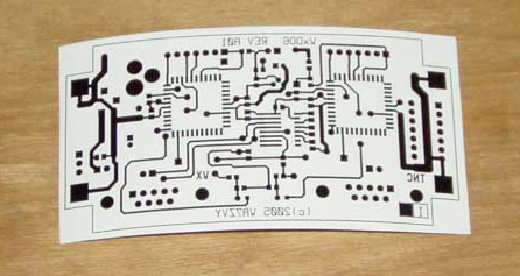
\includegraphics[width=0.45\textwidth]{images/pcb_on_paper.jpg}
    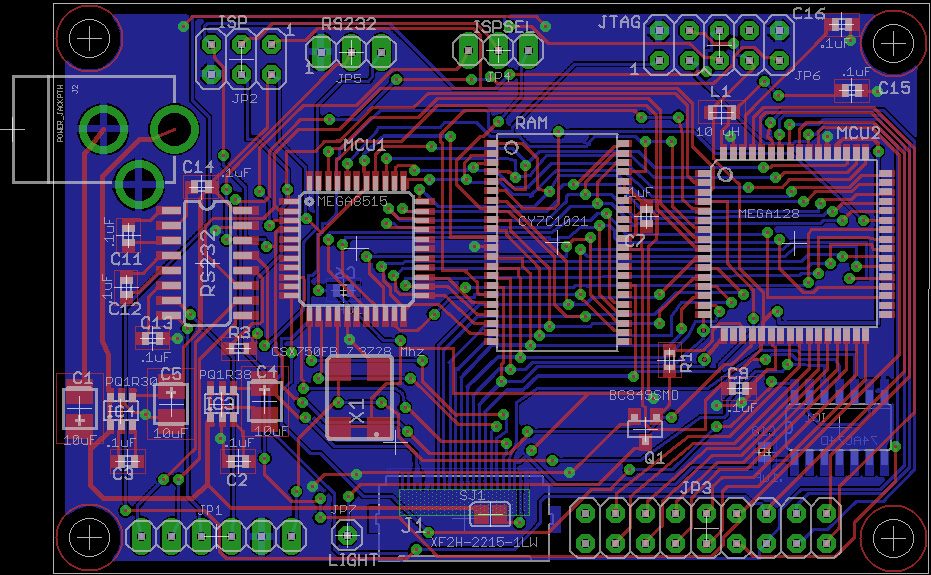
\includegraphics[width=0.45\textwidth]{images/pcb_in_kicad.jpg}
  \end{figure}
\end{frame}


%%%%%%%%%%%%%%%%%%%%%%%%%%%%%%%%%%%%%%%%%%%%%%%%%%%%%%%%%
\begin{frame}
  \frametitle{KiCAD}
  \begin{itemize}
    \item Developed by CERN
    \item Current version 4.0.*
    \item Next version (5.0) just around the corner
    \item Open ecosystem around components \& footprints
  \end{itemize}
\end{frame}


%%%%%%%%%%%%%%%%%%%%%%%%%%%%%%%%%%%%%%%%%%%%%%%%%%%%%%%%%
\begin{frame}
  \frametitle{Workflow}
  \begin{itemize}
    \item Schematics (represent Circuits)
    \item Associate Footprints
    \item Layout boards \& route traces
    \item Repeat for iterations
  \end{itemize}

  \begin{figure}[H]
    \centering
    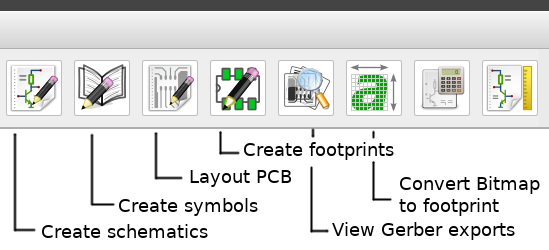
\includegraphics[width=0.95\textwidth]{images/workflow_overview.png}
  \end{figure}

\end{frame}


%%%%%%%%%%%%%%%%%%%%%%%%%%%%%%%%%%%%%%%%%%%%%%%%%%%%%%%%%
\begin{frame}
  \frametitle{Schematics}
  \begin{itemize}
    \item Symbols (Create missing symbols)
    \item Labels
    \item Connections
  \end{itemize}

  \begin{figure}[H]
    \centering
    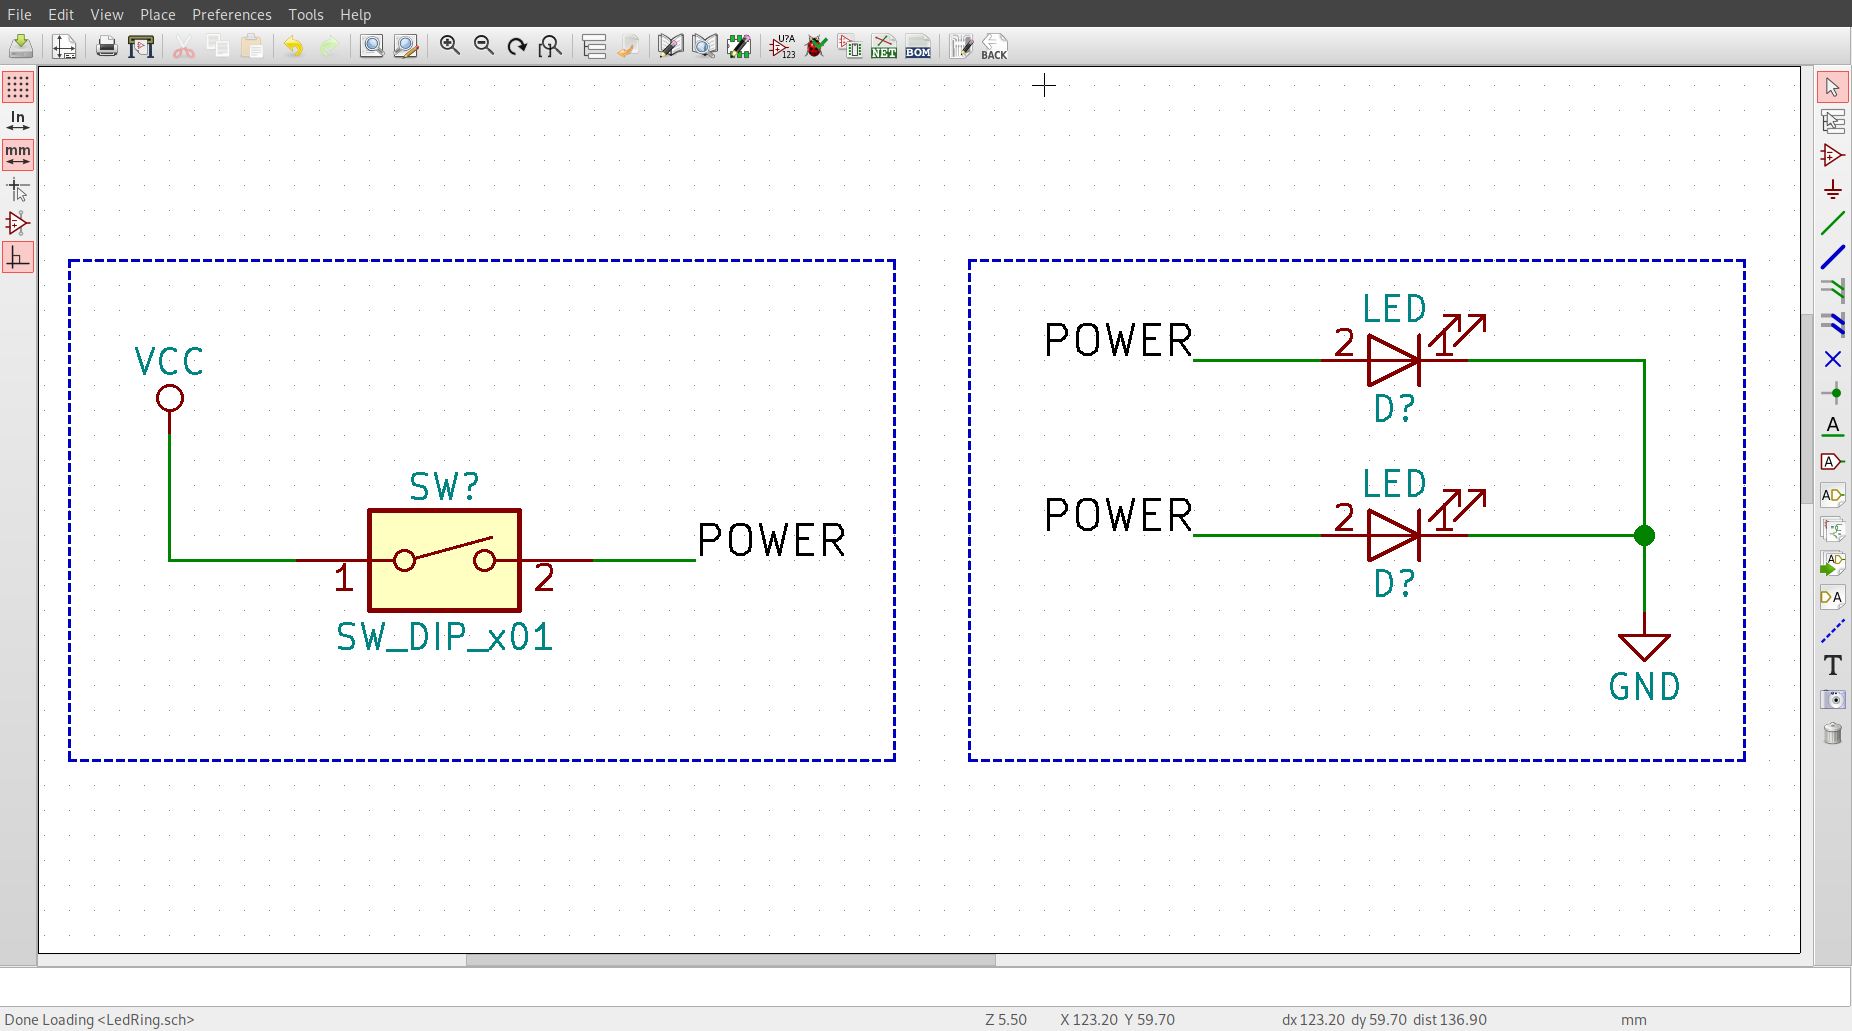
\includegraphics[width=0.95\textwidth]{images/kicad_schematic.png}
  \end{figure}

\end{frame}


%%%%%%%%%%%%%%%%%%%%%%%%%%%%%%%%%%%%%%%%%%%%%%%%%%%%%%%%%
\begin{frame}
  \frametitle{Schematics Workflow}
  \begin{itemize}
    \item Create circuit schematic
    \item Annotate (Give components unique names)
    \item Associate footprints
    \item Export Netlist
  \end{itemize}

  \begin{figure}[H]
    \centering
    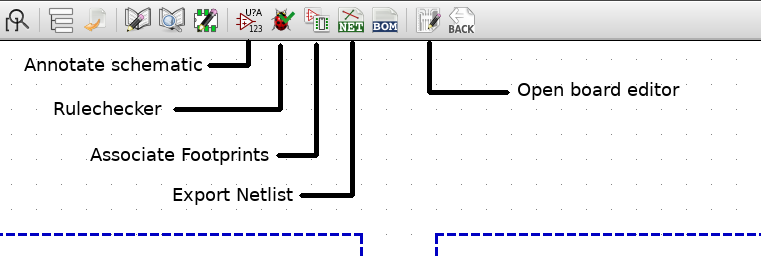
\includegraphics[width=0.95\textwidth]{images/kicad_schematic_workflow.png}
  \end{figure}
\end{frame}


%%%%%%%%%%%%%%%%%%%%%%%%%%%%%%%%%%%%%%%%%%%%%%%%%%%%%%%%%
\begin{frame}
  \frametitle{Board Layout}
  \begin{itemize}
    \item Import Netlist
    \begin{itemize}
      \item Imports component footprints
      \item Can replace/ update/ remove old footprints
      \item Import new Netlist for each revision
    \end{itemize}
    \item Layout components
    \item Route traces
    \item Export
    \begin{itemize}
      \item Gerber files (traces)
      \item Drill holes (holes, edge cuts)
      \item (Optional) Bill of Materials
    \end{itemize}
  \end{itemize}
\end{frame}


%%%%%%%%%%%%%%%%%%%%%%%%%%%%%%%%%%%%%%%%%%%%%%%%%%%%%%%%%
%%%%%%%%%%%%%%%%%%%%%%%%%%%%%%%%%%%%%%%%%%%%%%%%%%%%%%%%%
%%%%%%%%%%%%%%%%%%%%%%%%%%%%%%%%%%%%%%%%%%%%%%%%%%%%%%%%%


\begin{frame}
  \frametitle{Best Practises}
  \begin{itemize}
    \item Schematics
    \begin{itemize}
      \item Group components into segments (in nice boxes)
      \item Put large segments onto sub-sheets
      \item Use labels to connect segments together
    \end{itemize}
    
    \item Store required libraries in project
    \item Include datasheets for components

    \begin{figure}[H]
    \centering
    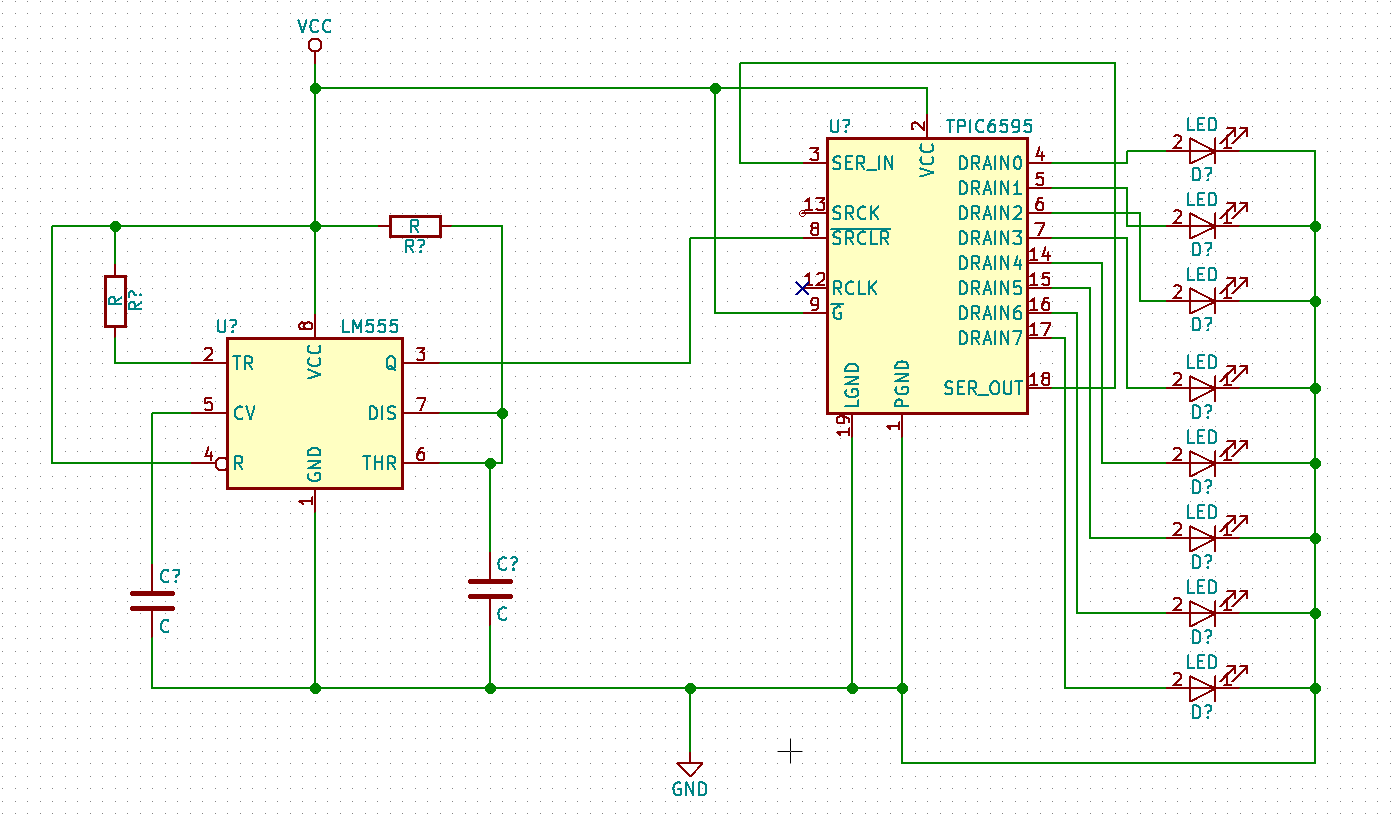
\includegraphics[width=0.50\textwidth]{images/kicad_schematic_bad.png}
    \caption{Avoid doing this!}
  \end{figure}
  \end{itemize}
\end{frame}


%%%%%%%%%%%%%%%%%%%%%%%%%%%%%%%%%%%%%%%%%%%%%%%%%%%%%%%%%
\begin{frame}
  \frametitle{Understanding Datasheets}
  \begin{itemize}
    \item Describes a component in detail
    \item Not everything always relevant
    \item Pick out important information
    \begin{itemize}
      \item High-level description
      \item Example usage
      \item Pin-out
      \item Footprint size
    \end{itemize}
  \end{itemize}
\end{frame}


%%%%%%%%%%%%%%%%%%%%%%%%%%%%%%%%%%%%%%%%%%%%%%%%%%%%%%%%%
\begin{frame}
  \frametitle{Finding Datasheets \& Components}
  \begin{itemize}
    \item Use component categories \& search on retail websites
    \begin{itemize}
      \item Farnell (Excellent search, medium catalogue)
      \item Digikey (Meh search, excellent catalogue)
      \item Mouser (Good search, good catalogue, expensive!)
      \item Adafruit (Limited catalogue, expensive!)
    \end{itemize}
    \item Datasheets provided by retail websites
    \item Often includes additional documentation
  \end{itemize}
\end{frame}



%%%%%%%%%%%%%%%%%%%%%%%%%%%%%%%%%%%%%%%%%%%%%%%%%%%%%%%%%
\begin{frame}
  \frametitle{Best Practises: Library Management}
  \begin{itemize}
    \item Three types of libraries
    \begin{itemize}
      \item Schematic symbols (.lib)
      \item Component footprints (.pretty)
      \item (Optional) 3D models (.3dshapes)
    \end{itemize}
    \item Different approaches to library management
    \begin{itemize}
      \item Each have their pro's and con's
      \item No "standard" way of doing it
      \item One library per ...
      \begin{itemize}
        \item Project
        \item Component type
        \item Manufacturer
        \item Individual component
      \end{itemize}
    \end{itemize}
  \end{itemize}
\end{frame}



\end{document}

